%%%%%%%%%%%%%%%%%%%%%%%%%%%%%%%%%%%%%%%%%%%%%%%%%%%%%%%%%%%%%%%%%%%%%%%%%%%%%%%%%%
\begin{frame}[fragile]\frametitle{}
\begin{center}
{\Large Introduction to Swift for Tensorflow}
\end{center}
\end{frame}


%%%%%%%%%%%%%%%%%%%%%%%%%%%%%%%%%%%%%%%%%%%%%%%%%%%%%%%%%%%%%%%%%%%%%%%%%%%%%%%%%%%
\begin{frame}[fragile]\frametitle{Quote}
\begin{lstlisting}
"I always hope that when I start looking at a new language, there will be some mind-opening new ideas to find, and Swift definitely doesn't disappoint. Swift tries to be expressive, flexible, concise, safe, easy to use, and fast. Most languages compromise significantly in at least one of these areas."

- Jeremy Howard
\end{lstlisting}
\end{frame}

%%%%%%%%%%%%%%%%%%%%%%%%%%%%%%%%%%%%%%%%%%%%%%%%%%%%%%%%%%%%%%%%%%%%%%%%%%%%%%%%%%%
\begin{frame}[fragile]\frametitle{Quote}
\begin{lstlisting}
"PyTorch was created to overcome the gaps in Tensorflow. FastAI was built to fill gaps in tooling for PyTorch. But now we're hitting the limits of Python, and Swift has the potential to bridge this gap"

- Jeremy Howard
\end{lstlisting}
\end{frame}

%%%%%%%%%%%%%%%%%%%%%%%%%%%%%%%%%%%%%%%%%%%%%%%%%%%
\begin{frame}[fragile] \frametitle{Swift for Tensorflow}

\begin{itemize}
\item Swift4Tensorflow isn’t just a Swift wrapper around TensorFlow but it’s being developed as a feature of the language itself. 
\item It is widely expected to become a core part of the language in the near future.
\item The library also adds many useful features to Swift like native support for automatic differentiation (which reminds me of Autograd in PyTorch) to make it even more compatible with numeric computing use-cases.
\end{itemize}

\begin{center}
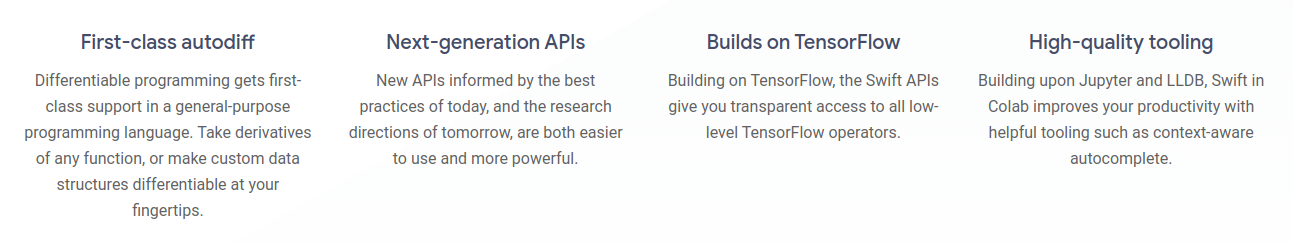
\includegraphics[width=\linewidth,keepaspectratio]{s4tf6}
\end{center}
\end{frame}


%%%%%%%%%%%%%%%%%%%%%%%%%%%%%%%%%%%%%%%%%%%%%%%%%%%%%%%%%%%%%%%%%%%%%%%%%%%%%%%%%%%
\begin{frame} \frametitle{Swift Ecosystem}
\begin{center}
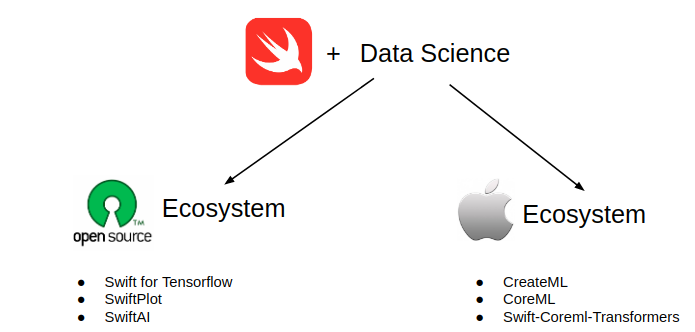
\includegraphics[width=0.9\linewidth,keepaspectratio]{s4tf2}
\end{center}

\begin{itemize}
\item Open-Source Swift runs on any machine.
\item For Apple ecosystem, need Apple machine to work on and you can only build for Apple devices like the iOS, macOS etc.
\end{itemize}

\end{frame}

%%%%%%%%%%%%%%%%%%%%%%%%%%%%%%%%%%%%%%%%%%%%%%%%%%%%%%%%%%%%%%%%%%%%%%%%%%%%%%%%%%%
\begin{frame} \frametitle{iOS/MacOS ML Apps}
\begin{center}
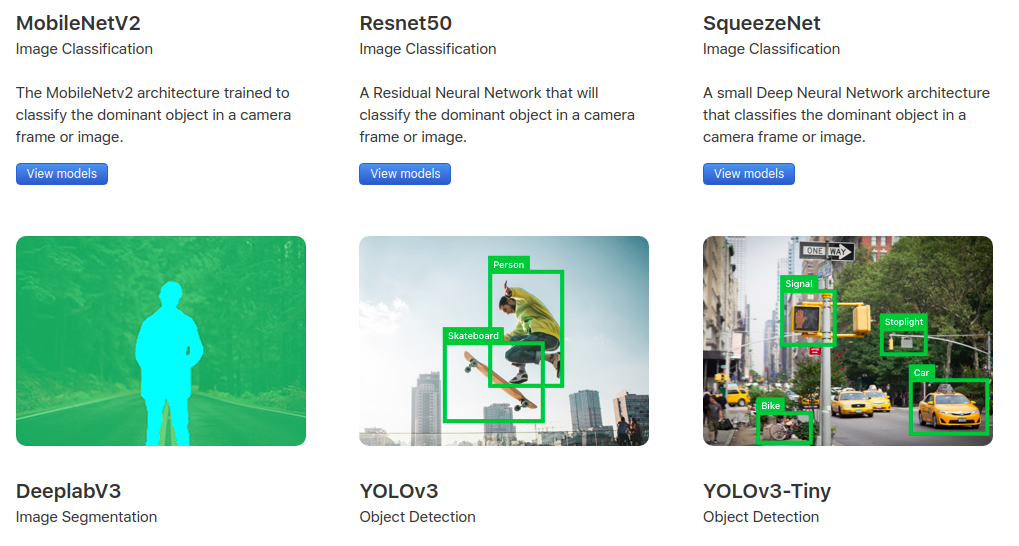
\includegraphics[width=0.9\linewidth,keepaspectratio]{s4tf3}
\end{center}
\end{frame}



%%%%%%%%%%%%%%%%%%%%%%%%%%%%%%%%%%%%%%%%%%%%%%%%%%%%%%%%%%%%%%%%%%%%%%%%%%%%%%%%%%%
\begin{frame} \frametitle{What is Swift for Tensorflow?}
\begin{center}
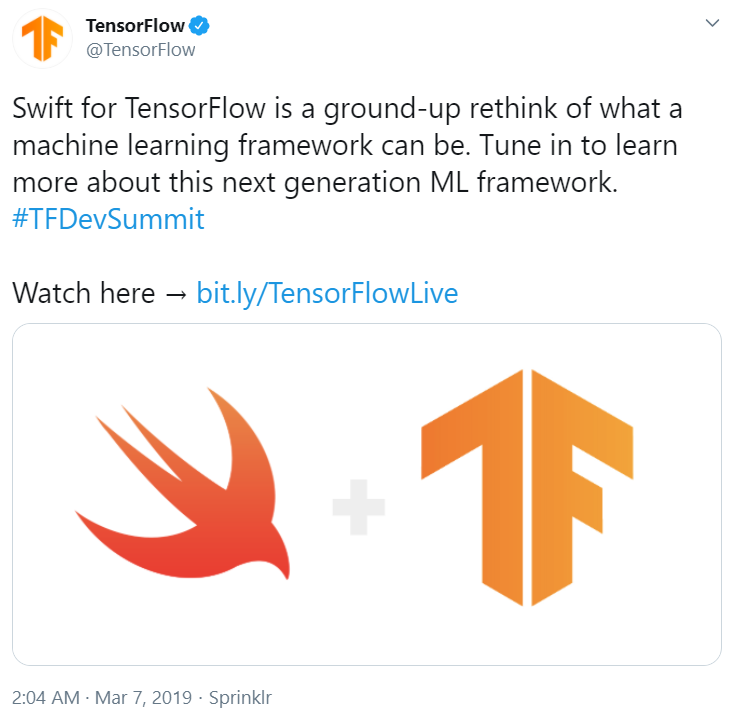
\includegraphics[width=0.65\linewidth,keepaspectratio]{s4tf1}
\end{center}
\end{frame}

%%%%%%%%%%%%%%%%%%%%%%%%%%%%%%%%%%%%%%%%%%%%%%%%%%%
\begin{frame}[fragile] \frametitle{MNIST with Swift for TensorFlow}


\begin{lstlisting}
var classifier = Sequential {
    Conv2D<Float>(filterShape: (5, 5, 1, 6), padding: .same, activation: relu)
    AvgPool2D<Float>(poolSize: (2, 2), strides: (2, 2))
    Conv2D<Float>(filterShape: (5, 5, 6, 16), activation: relu)
    AvgPool2D<Float>(poolSize: (2, 2), strides: (2, 2))
    Flatten<Float>()
    Dense<Float>(inputSize: 400, outputSize: 120, activation: relu)
    Dense<Float>(inputSize: 120, outputSize: 84, activation: relu)
    Dense<Float>(inputSize: 84, outputSize: 10, activation: softmax)
}
let optimizer = SGD(for: classifier, learningRate: 0.1)
\end{lstlisting}
\end{frame}

%%%%%%%%%%%%%%%%%%%%%%%%%%%%%%%%%%%%%%%%%%%%%%%%%%%
\begin{frame}[fragile] \frametitle{Future of Swift for Tensorflow}

\begin{itemize}
\item Currently, it is in infancy and the libraries around data science and numeric computing are still developing.
\item Has a strong industry backing behind it.
\item Swift will have a rich ecosystem of tools and libraries- maybe even better than what Python has today.
\end{itemize}

\end{frame}
